\documentclass[finnish, 11pt, fleqn]{beamer}
\usepackage{amsmath}
\usepackage{caption}
\usepackage{physics}
\usepackage{graphicx}
\usepackage{subcaption}
\usepackage{wrapfig}
\usepackage{mathtools}
\usepackage{xcolor}
\usepackage{listings}
\usepackage[font=footnotesize, labelfont=bf, justification=centering]{caption}

\renewcommand{\figurename}{Kuva}
\newcommand{\subitem}[1]{
    {\setlength\itemindent{15pt} \item[-] #1}
}


\makeatletter
\setbeamertemplate{frametitle}{
    \ifbeamercolorempty[bg]{frametitle}{}{\nointerlineskip}%
    \@tempdima=\textwidth%
    \advance\@tempdima by\beamer@leftmargin%
    \advance\@tempdima by\beamer@rightmargin%
    \begin{beamercolorbox}[sep=0.6cm,center,wd=\the\@tempdima]{frametitle}
        \usebeamerfont{frametitle}%
        \vbox{}\vskip-1ex%
        \if@tempswa\else\csname beamer@ftecenter\endcsname\fi%
        \strut\insertframetitle\strut\par%
        {%
            \ifx\insertframesubtitle\@empty%
            \else%
            {\usebeamerfont{framesubtitle}\usebeamercolor[fg]{framesubtitle}\insertframesubtitle\strut\par}%
            \fi
        }%
        \vskip-1ex%
        \if@tempswa\else\vskip-.3cm\fi% set inside beamercolorbox... evil here...
    \end{beamercolorbox}%
}
\makeatother

\beamertemplatenavigationsymbolsempty
\addtobeamertemplate{footline}{
    \usebeamercolor[fg]{title} 
    {\hspace{0.5em} \footnotesize Numeeriset menetelmät differentiaaliyhtälöille
    \hspace{1.5em} 21.2.2020
    \hspace{1.5em} Arttu Hyvönen}
    \hspace{2.0em} \large\insertframenumber/\inserttotalframenumber
}

\title{Numeeriset menetelmät differentiaaliyhtälöille\vspace{-3ex}}
\author{Arttu Hyv\"onen\vspace{-4ex}}
\date{21.2.2020\vspace{-2ex}}

\begin{document}

\begin{frame}[plain]
	\addtocounter{framenumber}{-2}
	\vspace{2em}
	\maketitle
	\begin{figure}[h!]
		\centering
		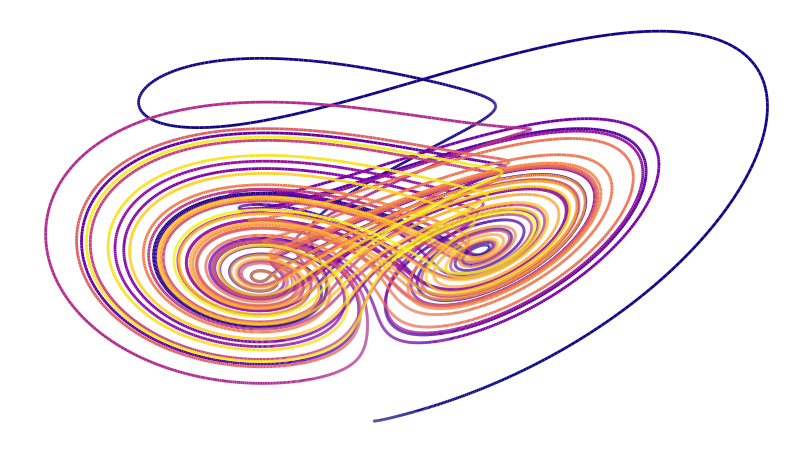
\includegraphics[scale=0.4]{graphics/attractor1.png}
		\\ {\small \caption{Chen attraktori Runge-Kutta menetelmällä}}
	\end{figure}
\end{frame}

\begin{frame}
    \frametitle{Sisältö}
    \begin{columns}[onlytextwidth]
		\begin{column}{.45\textwidth}
			\begin{figure}
				\vspace{-4em}
    			\begin{itemize}
    				\item{Yleistä tietoa aiheesta}
    				\item{Menetelmien esittely}
    					\subitem{Euler}
    					\subitem{Runge-Kutta}
    					\subitem{Leapfrog}
    				\item{Menetelmien vertailu}
    				\item{Yhteenveto}
    			\end{itemize}
			\end{figure}
		\end{column}
		\hfill
		\begin{column}{.45\textwidth}
			\begin{figure}
				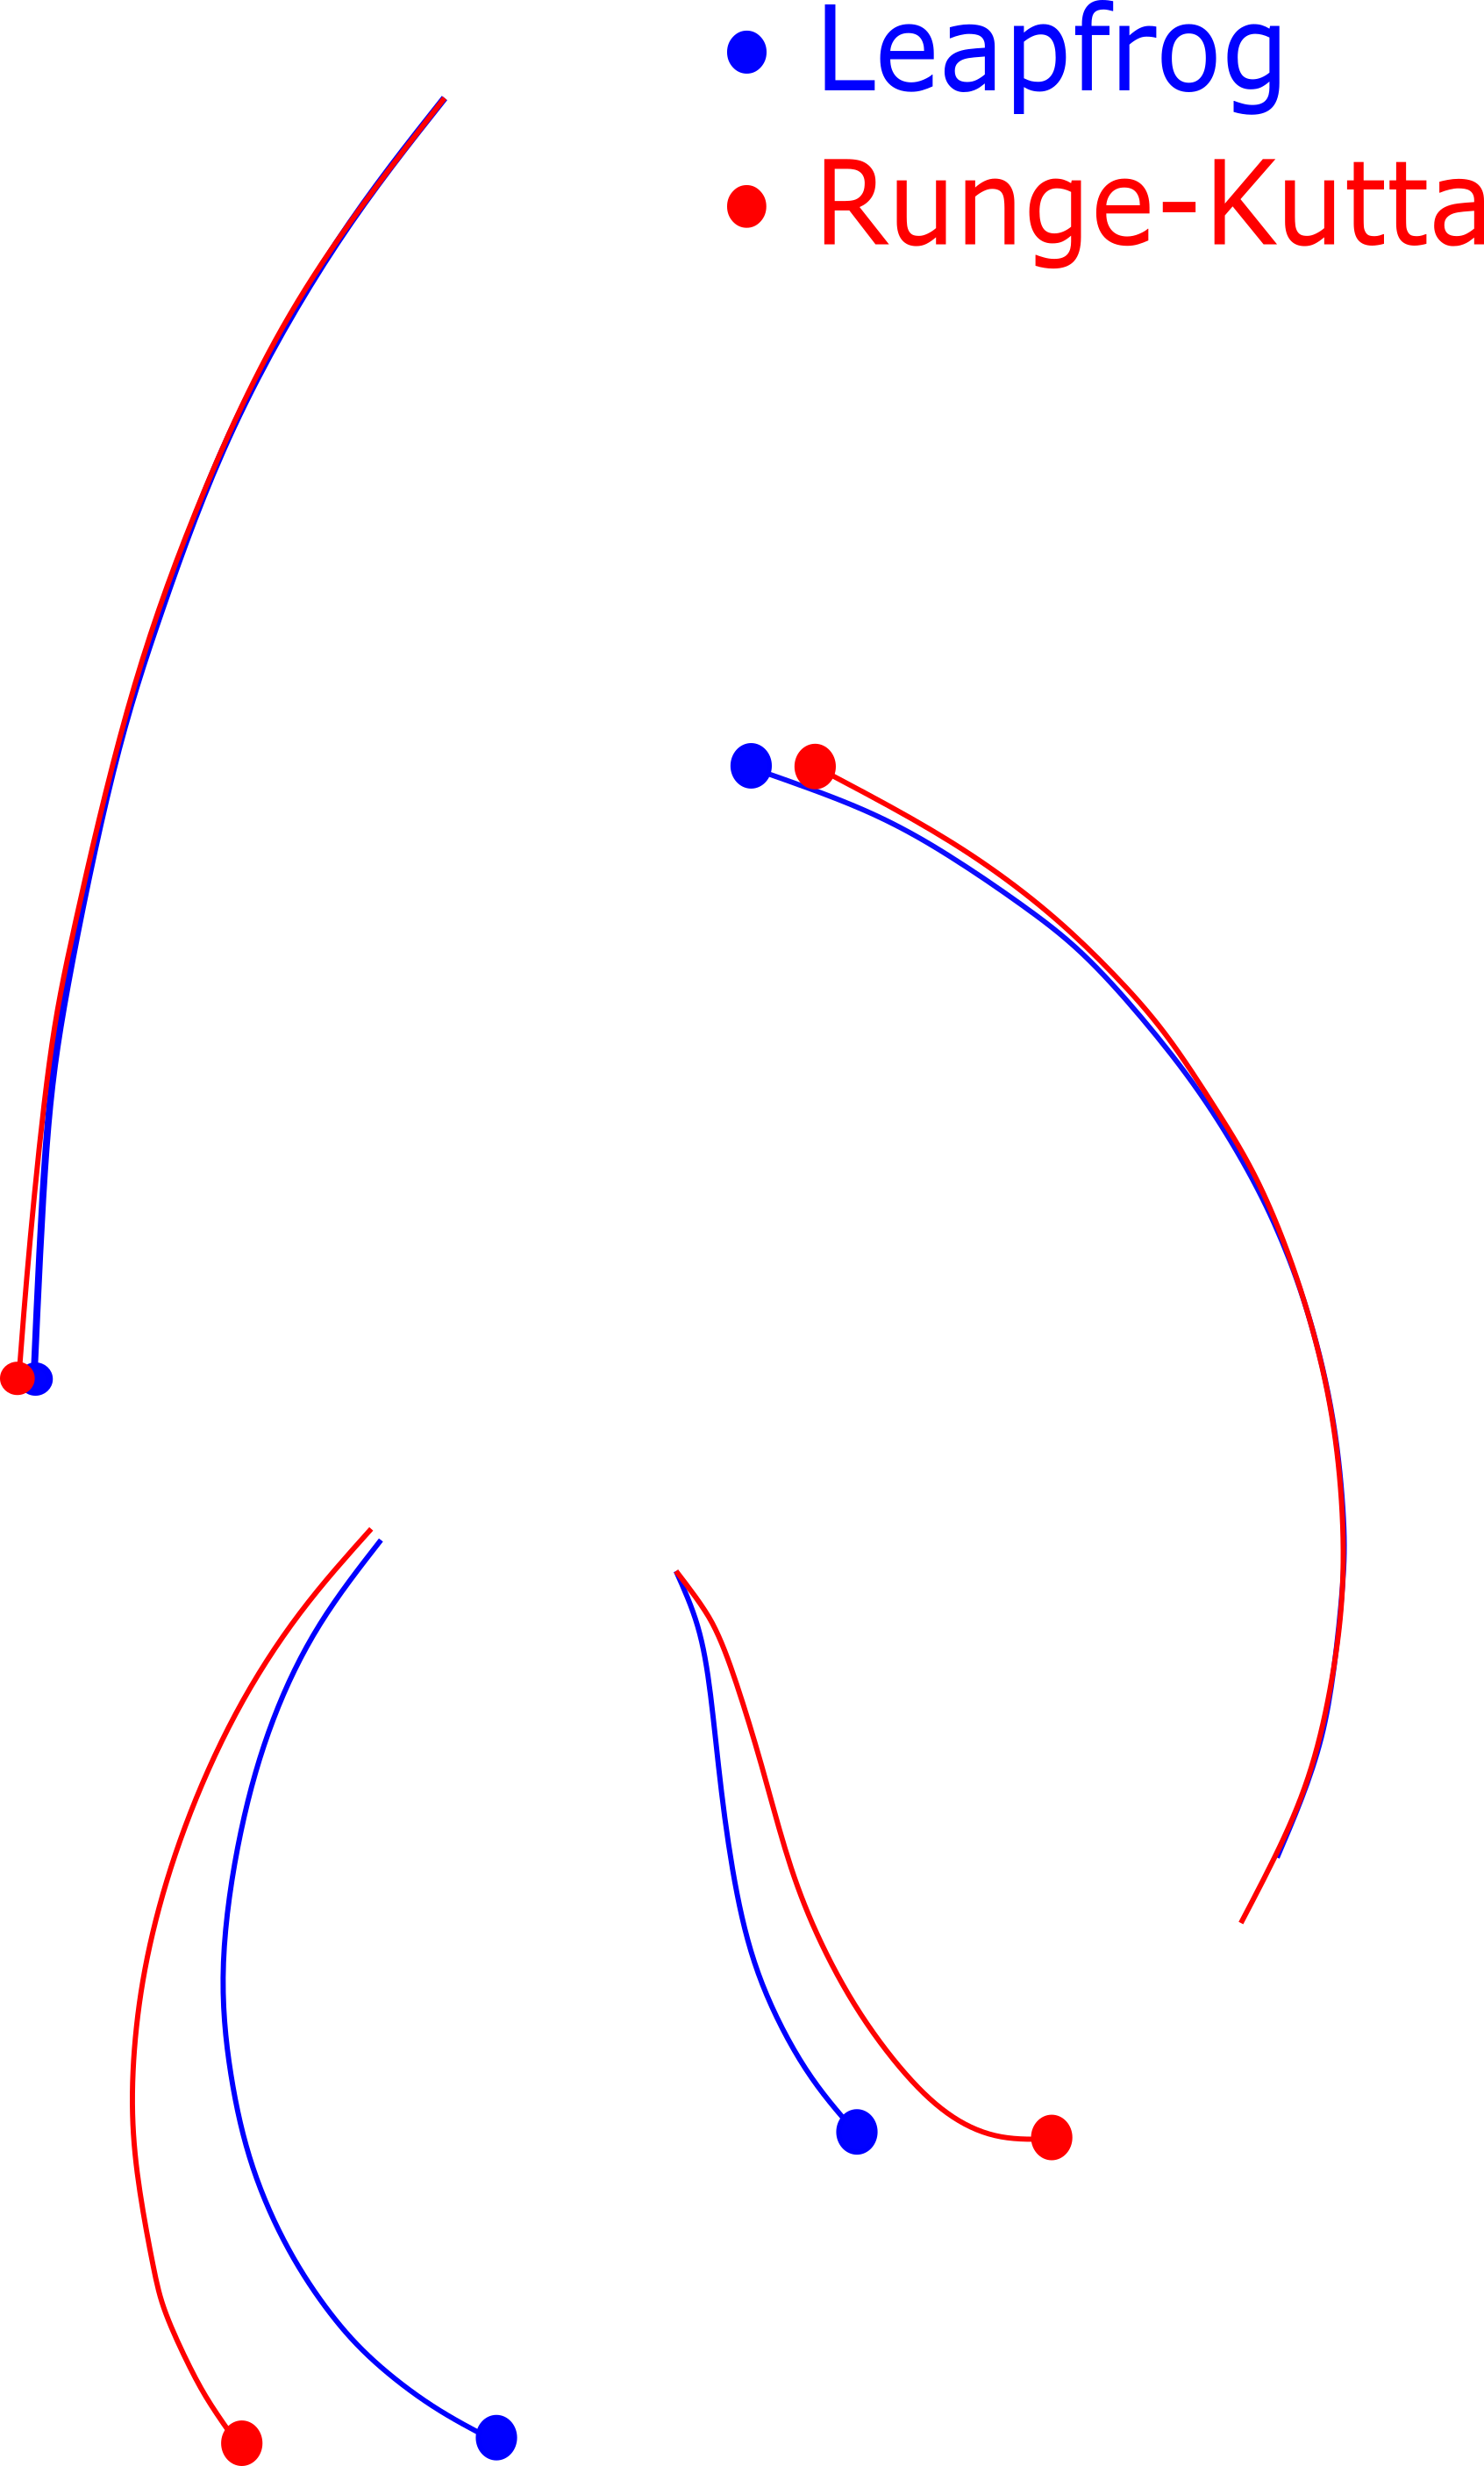
\includegraphics[scale=1.5]{graphics/tra_comp1.png}
				{\small \caption{Simulaatio gravitaatiosta eri menetelmillä}}
			\end{figure}
		\end{column}
	\end{columns}
    
\end{frame}

\begin{frame}
    \frametitle{Differentiaaliyhtälöt}
    \begin{columns}[onlytextwidth]
		\begin{column}{.45\textwidth}
			\begin{figure}
				\vspace{-4em}
    			\begin{itemize}
    				\item{Kuvaavat monenlaisia systeemejä}
    					\subitem{Populaatio}
    					\subitem{Kemialliset reaktiot}
    					\subitem{Pörssikurssit}
    				\item{Fysiikan matemaattisen muotoilun perusta}
    			\end{itemize}
			\end{figure}
		\end{column}
		\hfill
		\begin{column}{.55\textwidth}
			\begin{figure}[h!]
				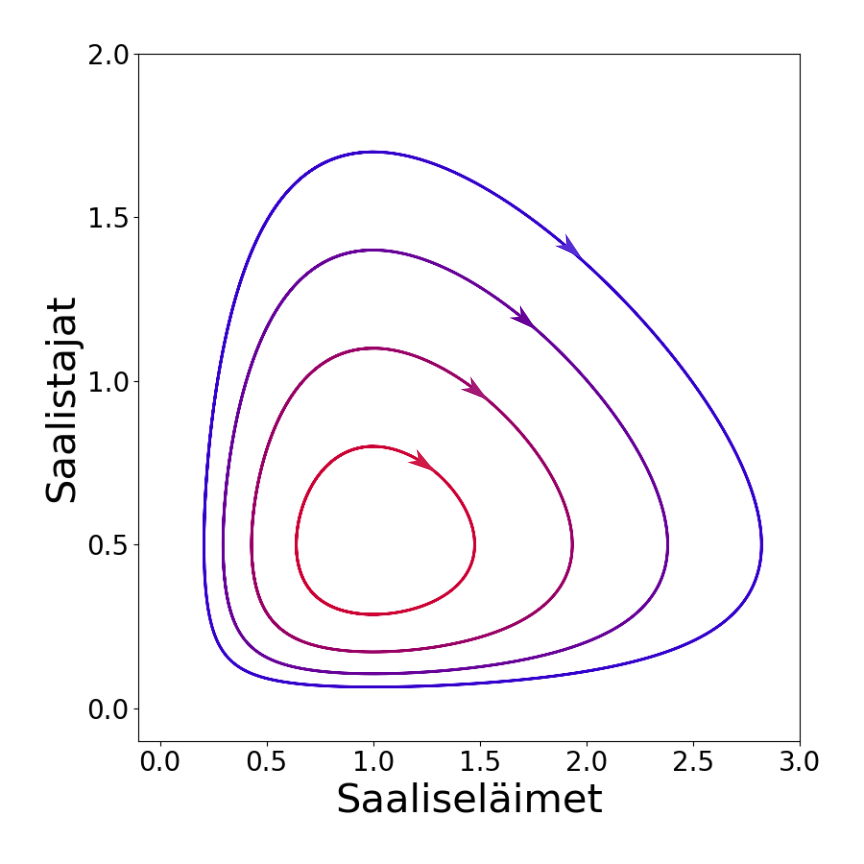
\includegraphics[scale=0.25]{graphics/lotka_volterra.png}
				{\caption{Populaation mallinnus Lotkan-Volterran yhtälöllä}}
			\end{figure}
		\end{column}
	\end{columns}	
\end{frame}

\begin{frame}
    \frametitle{Numeeristen menetelmien tarve}

		
	%\begin{align}
	%	\theta(t) &= 2 \arcsin\!\left\lbrace \! \sin\!\frac{\theta_0}{2} \, \mathrm{sn}\!\left[K\!\left(\sin^2\frac{\theta_0}{2}\right)\!-\omega_0 t, \, \sin^2\!\frac{\theta_0}{2}\right]\!\right\rbrace \\
	%	\mathrm{sn}(u, k) &=  \frac{\vartheta(0, \tau)}{\vartheta(0, \tau)} \:\frac{\vartheta_{10}[u \, \vartheta(0, \tau)^{-2}, \tau]}{\vartheta[u \, \vartheta(0, \tau)^{-2} + \frac{1}{2}, \tau]} \\ 
	%	\vartheta(z, \tau) &= \sum_{n=-\infty}^{\infty} \exp(\pi i n^2 \tau + 2\pi i n z) 
	%\end{align}

	%{\small \hspace{1em} \textbf{Kaava:} Heilurin yhtälö ja analyyttinen ratkaisu}
		\begin{columns}[onlytextwidth]
		\begin{column}{.45\textwidth}
			\begin{figure}
    			\begin{itemize}
    				\vspace{-4em}
    				\item{Kaikki yhtälöt eivät ratkea analyyttisesti}
    				\vspace{1em}
    				\item{Ratkaisu saattaa olla liian kömpelö käyttää}
    			\end{itemize}
			\end{figure}
		\end{column}
		\hfill
		\begin{column}{.55\textwidth}
			\begin{figure}[h!]
				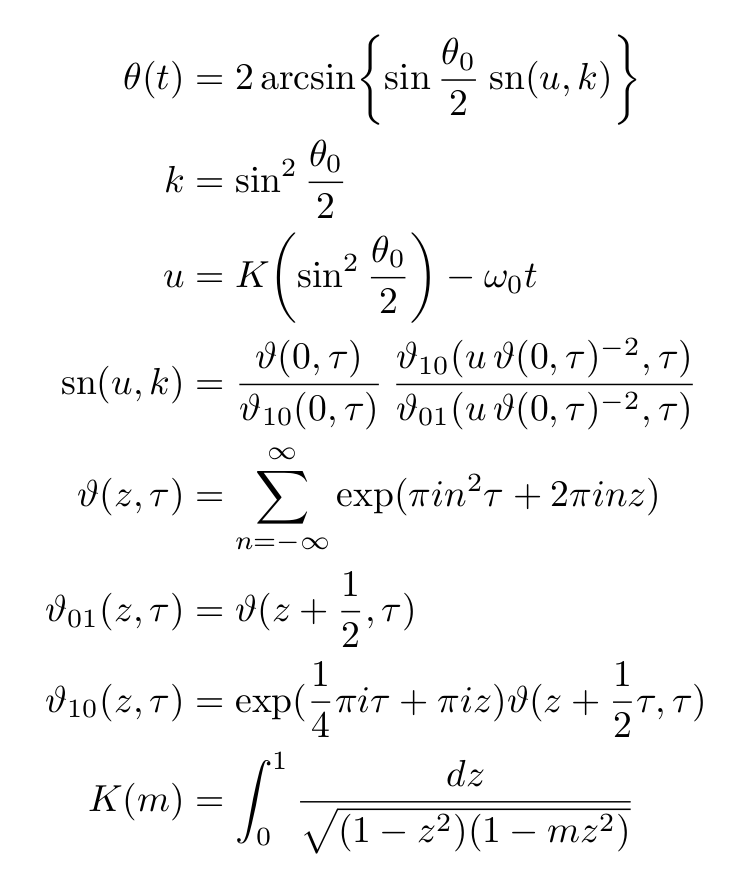
\includegraphics[scale=0.25]{graphics/kaava.png}
				{\caption{Heilurin analyyttinen ratkaisu ja funktioiden määritelmät}}
			\end{figure}
		\end{column}
	\end{columns}
	
\end{frame}

\begin{frame}
    \frametitle{Numeeristen menetelmien tavoite}
	\begin{itemize}
    	\vspace{-2em}
    	\item{Tavoite on ottaa differentiaaliyhtälö ja ratkaista siitä haluttu muuttuja}
    	\vspace{1em}
    	$$\dfrac{dy}{dt} = f(t, y) \: \rightarrow \: y = g(t)$$
    	\vspace{0.5 em}
    	\item{Tähän päästään ottamalla alkuarvo ja laskemalla loput arvot yhtälön mukaan}
    \end{itemize}
\end{frame}

\begin{frame}
	\frametitle{Eulerin menetelmä}
	\begin{columns}[onlytextwidth]
		\begin{column}{.45\textwidth}
			\begin{figure}
				\vspace{-4em}
    			\begin{itemize}
    				\item{Yksinkertaisin menetelmä}
    				\vspace{0em}
    				\item{Helppo toteuttaa, mutta epätarkka}
					\vspace{1em}    				
    				\item{Toimii pohjana tarkemmille menetelmille}
    			\end{itemize}
			\end{figure}
		\end{column}
		\hfill
		\begin{column}{.55\textwidth}
			\begin{figure}[h!]
				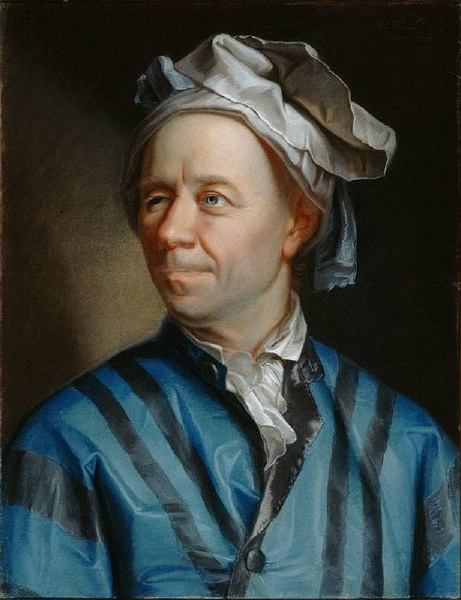
\includegraphics[scale=0.25]{graphics/Leonhard_Euler.jpg}
				{\caption{Leonhard Euler}}
			\end{figure}
		\end{column}
	\end{columns}	
\end{frame}

\begin{frame}
	\frametitle{Eulerin menetelmän toiminta}
	\begin{columns}[onlytextwidth]
		\begin{column}{.45\textwidth}
			\begin{figure}
				\vspace{-4em}
    			\begin{enumerate}
    				\item{\small Alkuarvo \normalsize $y_n$}
    				\vspace{1em}
    				\item{\small Funktio kulmakertoimelle \normalsize $\dfrac{dy}{dt} = k(t)$}
					\vspace{1em}
    				\item{\small Edetään askel $h$ kerrallaan}
    				$y_{n+1} = y_n + h\,k(t_n)$
    			\end{enumerate}
			\end{figure}
		\end{column}
		\hfill
		\begin{column}{.55\textwidth}
			\begin{figure}[h!]
				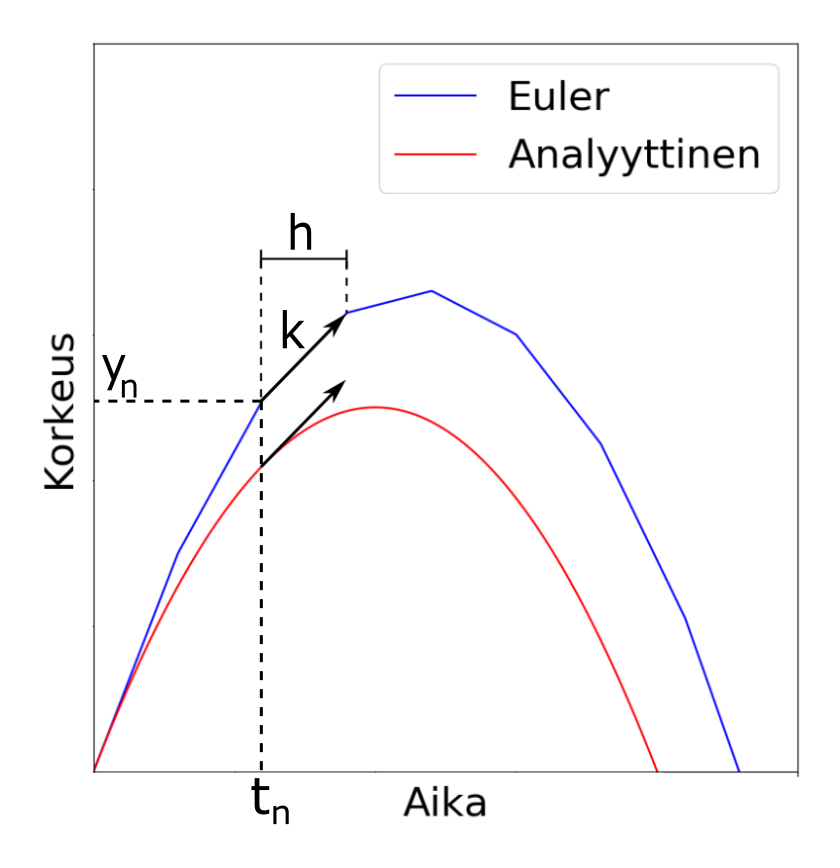
\includegraphics[scale=0.25]{graphics/Euler_1.png}
				{\caption{Heitetyn pallon korkeus ajan funktiona}}
			\end{figure}
		\end{column}
	\end{columns}	
\end{frame}

\begin{frame}
	\frametitle{Runge-Kutta menetelmät}
	\begin{columns}[onlytextwidth]
		\begin{column}{.5\textwidth}
			\begin{figure}
				\vspace{-2em}
    			\begin{itemize}
    				\item{\small Joukko menetelmiä jotka kehitettiin 1900 alussa}
    				\vspace{1em}
    				\item{\small Yhden kulmakertoimen sijasta lasketaan monta}
    				\vspace{1em}
    				\item{\small Tunnetuimmasta menetelmästä käytetään nimeä Runge-Kutta menetelmä}
    			\end{itemize}
			\end{figure}
		\end{column}
		\hfill
		\begin{column}{.45\textwidth}
			\begin{figure}[t!]
    			\centering
    			\begin{subfigure}[t]{0.5\textwidth}
        			\centering
        			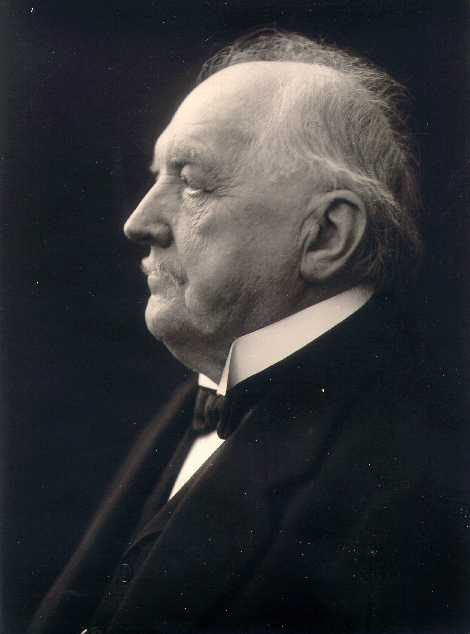
\includegraphics[height=1.6in]{graphics/Martin_Wilhelm_Kutta.jpg}
    			\end{subfigure}%
    			~
    			\begin{subfigure}[t]{0.5\textwidth}
        			\centering
        			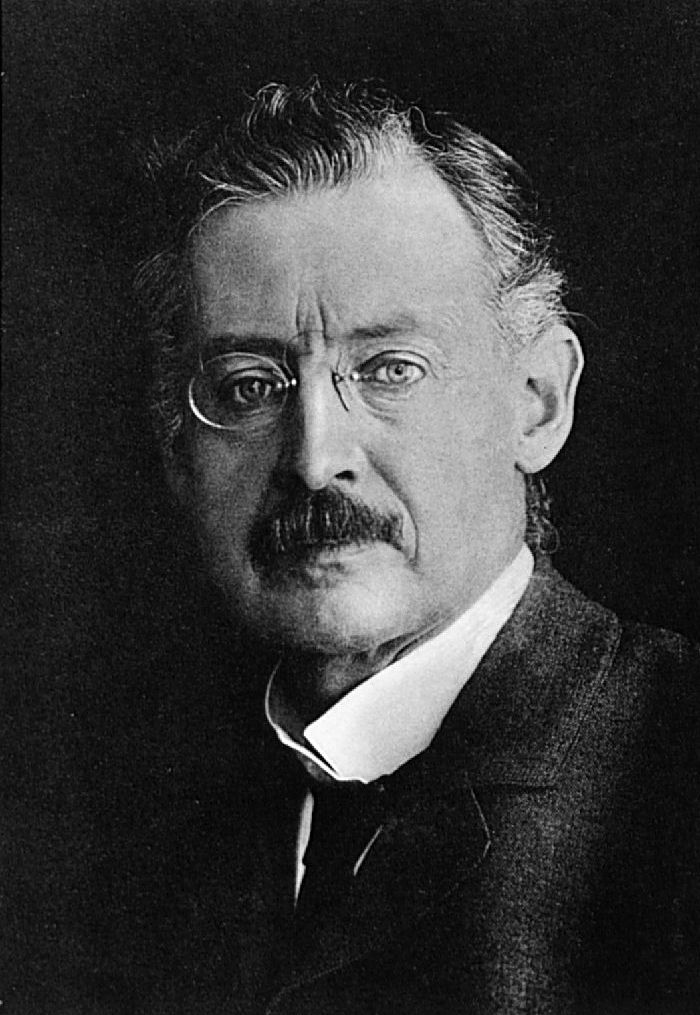
\includegraphics[height=1.6in]{graphics/Karl_Runge.jpg}
    			\end{subfigure}
    			\caption{Martin Kutta ja Carl Runge}
			\end{figure}
		\end{column}
	\end{columns}	
\end{frame}

\begin{frame}
	\frametitle{Runge-Kutta menetelmän toiminta}
	\vspace{-2em}	
	\begin{columns}[onlytextwidth]
		\begin{column}{.35\textwidth}
			\begin{figure}
				\vspace{-2em}
    			\begin{enumerate}
    				\item{\small Alkuarvo $y_n$}
    				\vspace{1em}
    				\item{\small Lasketaan kulmakertoimet $k_1, ... k_4$}
					\vspace{1em}    				
    				\item{\small Edetään askel $h$}
    			\end{enumerate}
    			\hspace{0em} $y_{n+1} = y_n + h\,K$
			\end{figure}
		\end{column}
		\hfill
		\begin{column}{.65\textwidth}
			\begin{figure}[h!]
				\vspace{-1em}
				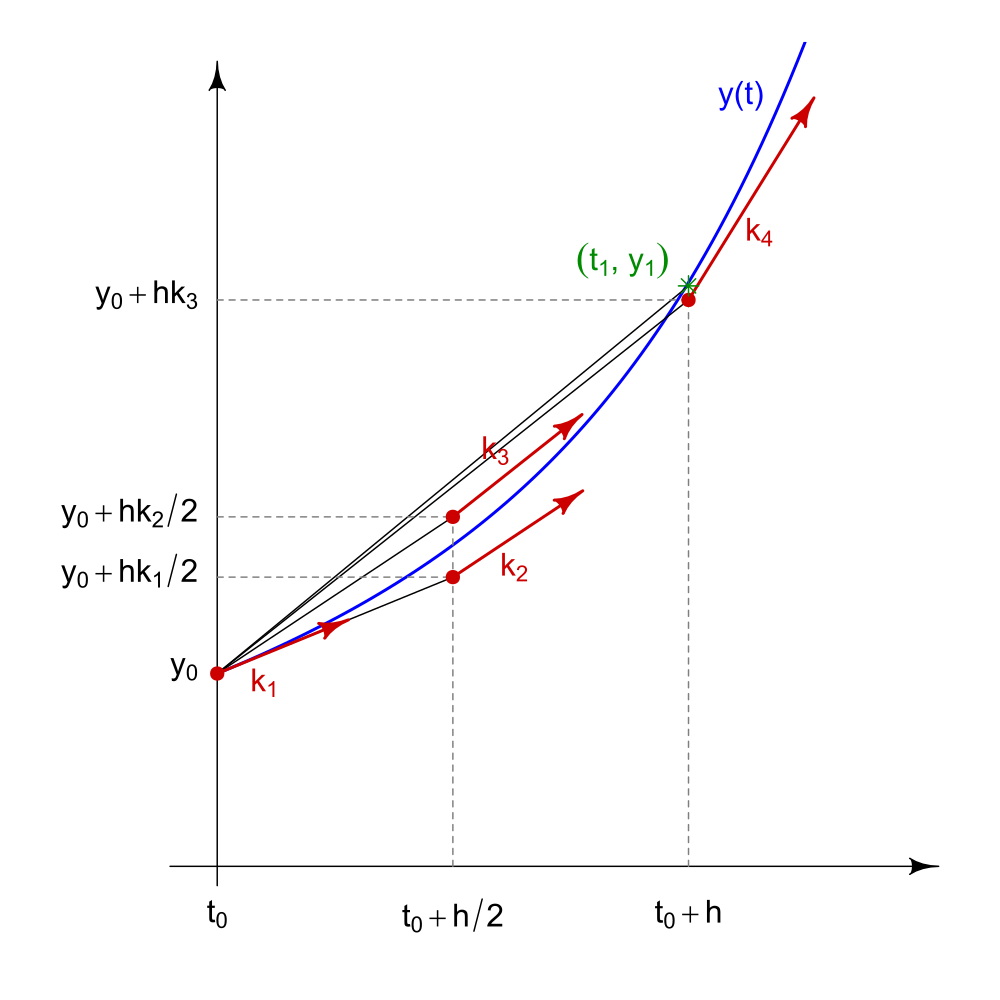
\includegraphics[scale=0.22]{graphics/Runge-Kutta_slopes.png}
				\vspace{-2.5em}				
				{\caption{Askel Runge-Kutta menetelmällä}}
			\end{figure}
		\end{column}
	\end{columns}	
\end{frame}

\begin{frame}
	\frametitle{Leapfrog menetelmä}
	\begin{columns}[onlytextwidth]
		\begin{column}{.45\textwidth}
			\begin{figure}
				\vspace{-3em}
    			\begin{itemize}
    				\item{Toimii yhtälöille muotoa $\dfrac{d^2y}{dt^2} = a(t, y)$}
    				\vspace{1.5em}
    				\item{Säilyttää fysikaalisen systeemin kokonaisenergian}
    				\subitem{Epätarkkuutta \\}
    				\hspace{1.1em} muualla
    			\end{itemize}
			\end{figure}
		\end{column}
		\hfill
		\begin{column}{.55\textwidth}
			\begin{figure}[h!]
				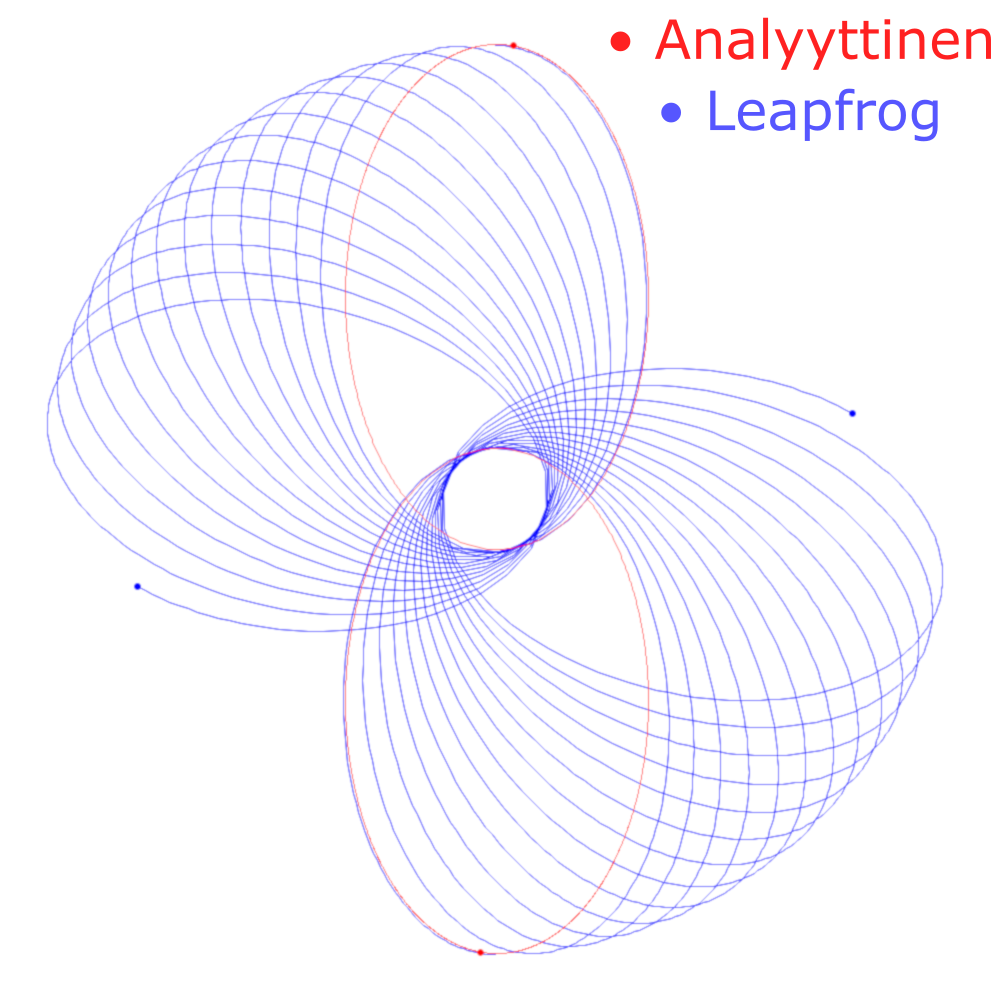
\includegraphics[scale=0.7]{graphics/2kpl_prek.png}
				{\caption{Kahden kappaleen simulaatio}}
			\end{figure}
		\end{column}
	\end{columns}	
\end{frame}

\begin{frame}
	\frametitle{Leapfrog menetelmän toiminta}
	\vspace{1em}
	\begin{enumerate}
		\item{Alkuarvot paikalle $y_0$ ja nopeudelle $v_{1/2}$}
		\vspace{0.5em}
		\item{Funktio kiihtyvyydelle $a(t_n, y_n)\equiv a_n$}
		\vspace{0.5em}
		\item{\small Edetään askel $h$ eteenpäin $y$:llä ja $v$:llä}
	\end{enumerate}
	\vspace{1em}
	\begin{figure}[h!]
		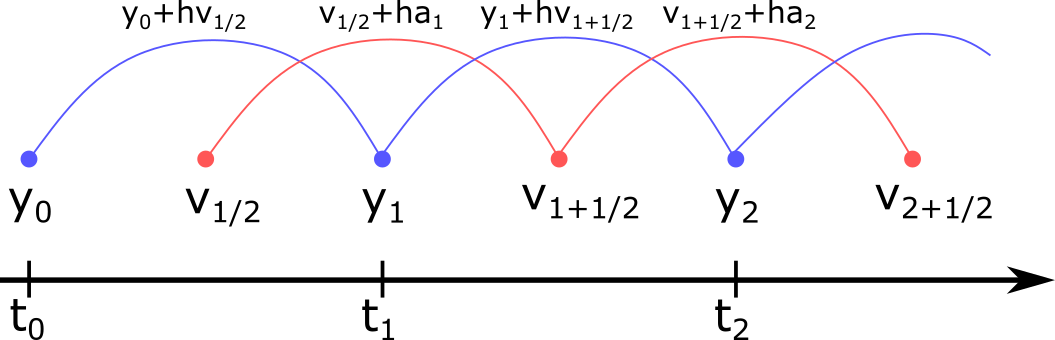
\includegraphics[scale=0.6]{graphics/leapfrog_ult.png}	
		{\caption{Ensimmäiset askeleet Leapfrog menetelmällä}}
	\end{figure}
\end{frame}

\begin{frame}[fragile]
	\frametitle{Menetelmien toteutus koodina}
	\begin{columns}[onlytextwidth]
		\begin{column}{.3\textwidth}
			{\tiny
			{\small \textcolor{blue}{Eulerin menetelmä}}
			\begin{lstlisting}
def euler(h, t, q0, p0, dq, dp):
    k1 = dq(t, q0, p0)
    l1 = dp(t, q0, p0)
	
    q1 = q0 + k1*h
    p1 = p0 + l1*h
    				
    return [q1, p1]
			\end{lstlisting}
			\vspace{1em}
			{\small \textcolor{blue}{Leapfrog menetelmä}}
			\begin{lstlisting}
def leapfrog(h, t, q0, p0, ddq):
    p12 = p0 + ddq(t, q0)*h*0.5
    q1 = q0 + p12*h
    p1 = p12 + ddq(t, q1)*h*0.5
    
    return [q1, p1]
			\end{lstlisting}}
		\end{column}
		\hfill
		\begin{column}{.5\textwidth}
			\vspace{-1.5em}			
			\begin{figure}[h!]
			{\tiny
			{\small \hspace{-5.5em} \textcolor{blue}{Runge-Kutta menetelmä}}
			\begin{lstlisting}
def rk4(h, t, q0, p0, dq, dp):
    k1 = h*dq(t, q0, p0)
    l1 = h*dp(t, q0, p0)

    k2 = h*dq(t+0.5*h, q0+0.5*k1, p0+0.5*l1)
    l2 = h*dp(t+0.5*h, q0+0.5*k1, p0+0.5*l1)

    k3 = h*dq(t+0.5*h, q0+0.5*k2, p0+0.5*l2)
    l3 = h*dp(t+0.5*h, q0+0.5*k2, p0+0.5*l2)

    k4 = h*dq(t+h, q0+k3, p0+l3)
    l4 = h*dp(t+h, q0+k3, p0+l3)

    q1 = q0 + (k1 + 2*k2 + 2*k3 + k4)/6.0
    p1 = p0 + (l1 + 2*l2 + 2*l3 + l4)/6.0

    return [q1, p1]
			\end{lstlisting}}
			\end{figure}
		\end{column}
	\end{columns}
\end{frame}

\begin{frame}
	\frametitle{Vertailu systeemi}
	\begin{columns}[onlytextwidth]
		\begin{column}{.5\textwidth}
			\begin{figure}
				\vspace{-3em}
    			\begin{itemize}
    				\item{Systeeminä käytetään ideaalista heiluria}
    				\vspace{0.5em}
    				\item{Leapfrog\\}
    				\vspace{0.5em}
    				\hspace{-2.0em}$\dfrac{d^2\theta(t)}{dt^2} = -\sin(\theta)$
    				\vspace{1.0em}
    				\item{Runge-Kutta, Euler\\}
    				\vspace{0.5em}
    				\hspace{-2.0em}$\dfrac{dp_{\theta}(t)}{dt} = -\sin(\theta), \: \dfrac{d\theta}{dt} = p_{\theta}$
    			\end{itemize}
			\end{figure}
		\end{column}
		\hfill
		\begin{column}{.55\textwidth}
			\vspace{-1.5em}			
			\begin{figure}[h!]
				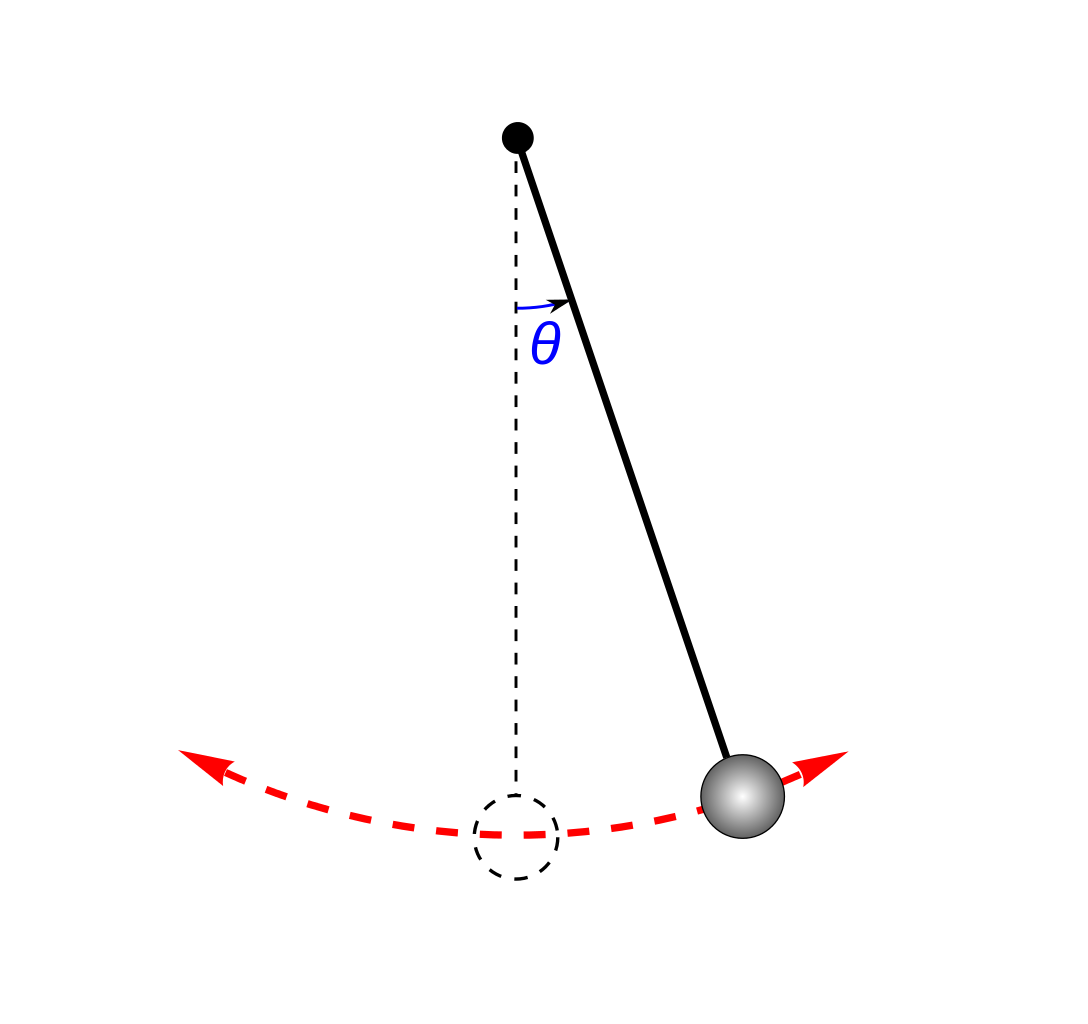
\includegraphics[scale=0.7]{graphics/pendulum.png}
				\vspace{-2.5em}				
				{\caption{Heiluri}}
			\end{figure}
		\end{column}
	\end{columns}
\end{frame}

\begin{frame}
	\frametitle{Runge-Kutta ja Euler mentelmät}
	\begin{columns}[onlytextwidth]
		\begin{column}{.3\textwidth}
			\begin{figure}
				\vspace{-2.5em}
    			\begin{itemize}
    				\item{Runge-Kutta ja analyyttinen lähes identtiset}
    				\vspace{0.5em}
    				\item{Eulerin menetelmällä kasaantuu virhettä}
    			\end{itemize}
			\end{figure}
		\end{column}
		\hfill
		\begin{column}{.65\textwidth}
			\vspace{-1.5em}			
			\begin{figure}[h!]
				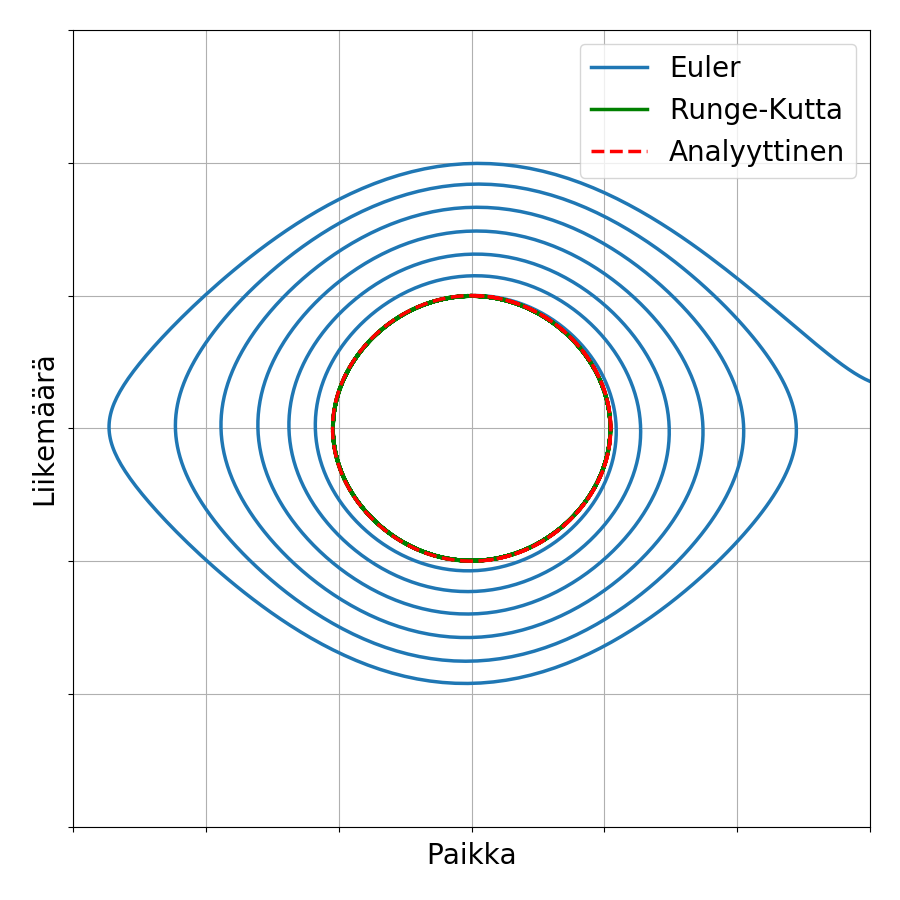
\includegraphics[scale=0.32]{graphics/comp2.png}
				\vspace{-2.5em}				
				%{\caption{Heiluri}}
			\end{figure}
		\end{column}
	\end{columns}
\end{frame}

\begin{frame}
	\frametitle{Runge-Kutta ja Leapfrog mentelmät}
	\vspace{-1em}
	\begin{figure}[h!]
		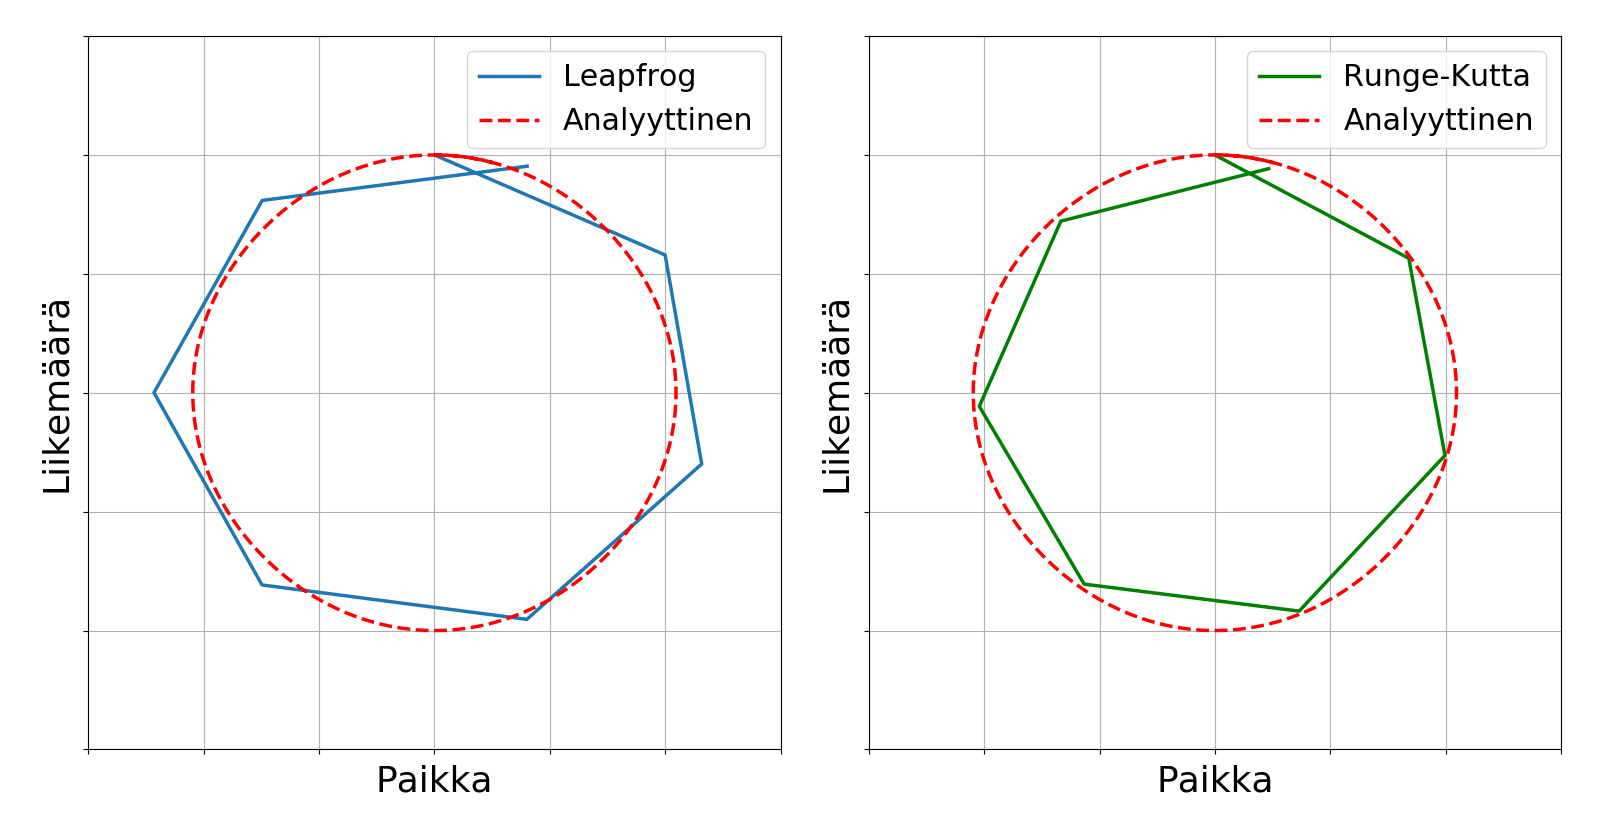
\includegraphics[scale=0.27]{graphics/comp3.png}	
		{\caption{Yksi heilahdus Runge-Kutta ja Lepafrog menetelmillä}}
	\end{figure}
\end{frame}

\begin{frame}
	\frametitle{Runge-Kutta ja Leapfrog mentelmät}
	\vspace{-1em}
	\begin{figure}[h!]
		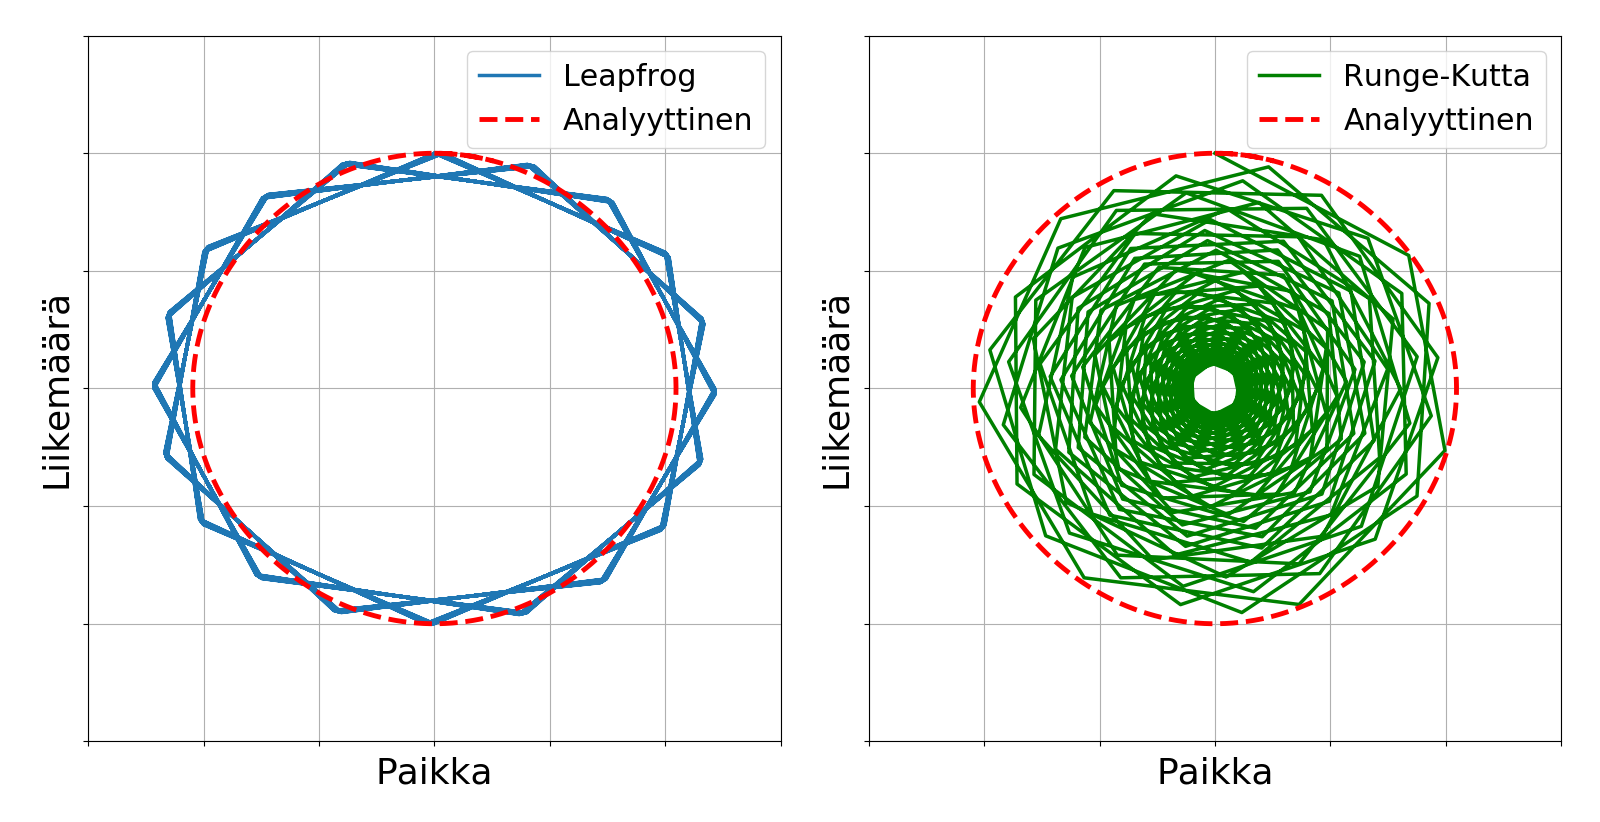
\includegraphics[scale=0.27]{graphics/comp4.png}	
		{\caption{Monta heilahdusta Runge-Kutta ja Leapfrog menetelmillä}}
	\end{figure}
\end{frame}

\begin{frame}
	\frametitle{Runge-Kutta ja Leapfrog mentelmät}
	\vspace{-1em}
	\begin{figure}[h!]
		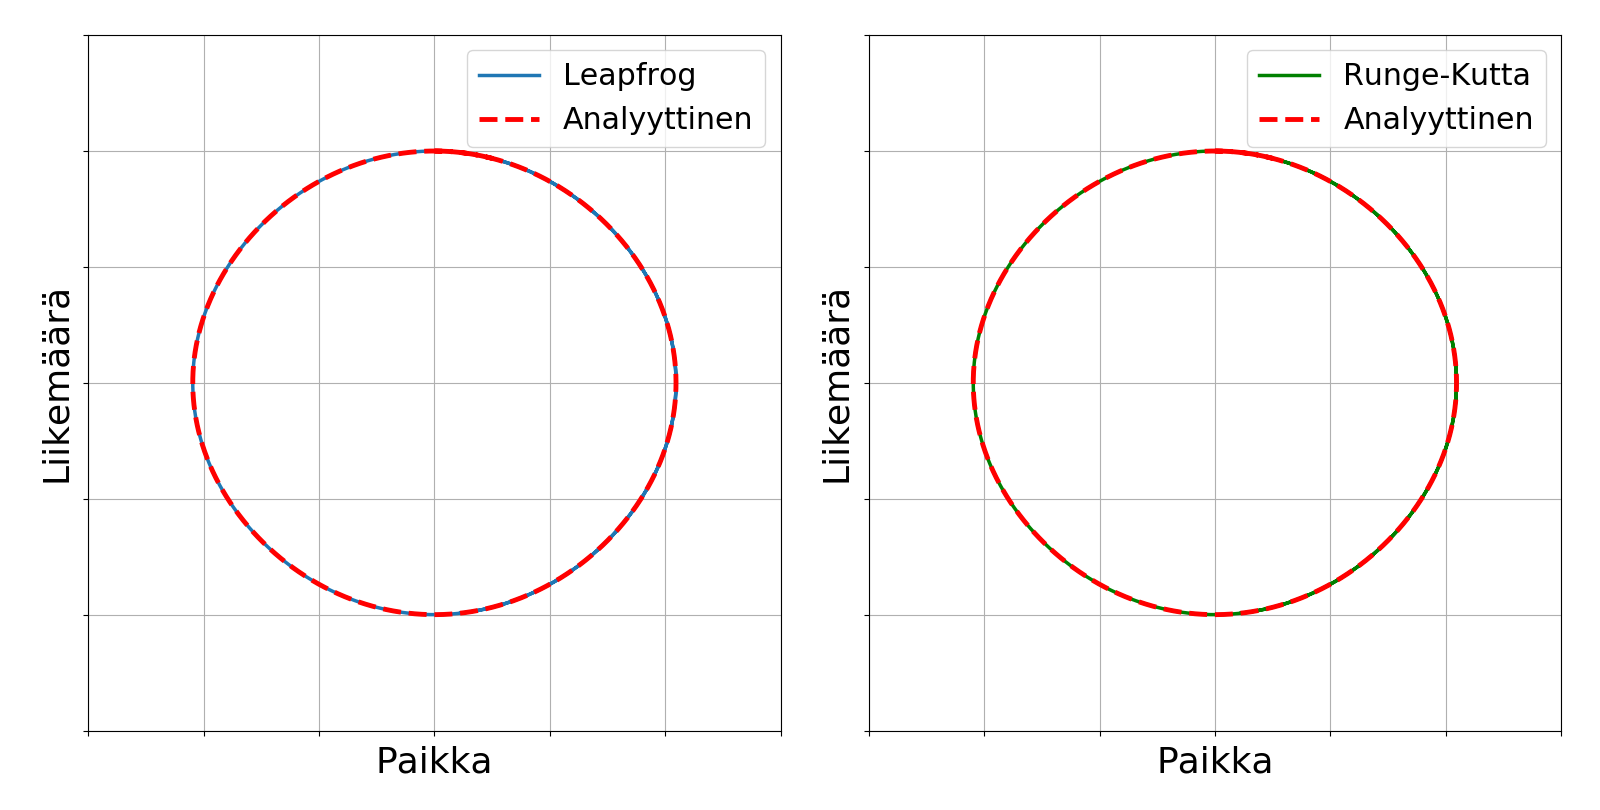
\includegraphics[scale=0.27]{graphics/comp5.png}	
		{\caption{Monta heilahdusta pienellä aika-askeleella}}
	\end{figure}
\end{frame}

\begin{frame}
	\frametitle{Yhteenveto}
    \begin{columns}[onlytextwidth]
		\begin{column}{.42\textwidth}
			\begin{figure}
				\vspace{-3em}
    			\begin{itemize}
    				\item{Eulerin menetelmä on epätarkka}
    				\vspace{0.5em}
    				\item{Leapfrog on tarkka ja nopea mutta sen käytöllä on rajoituksia}
					\vspace{0.5em}    				
    				\item{Runge-Kutta on melko tarkka ja sitä voi käyttää monissa tilanteissa}
    			\end{itemize}
			\end{figure}
		\end{column}
		\hfill
		\begin{column}{.55\textwidth}
			\vspace{-1em}
			\begin{figure}
				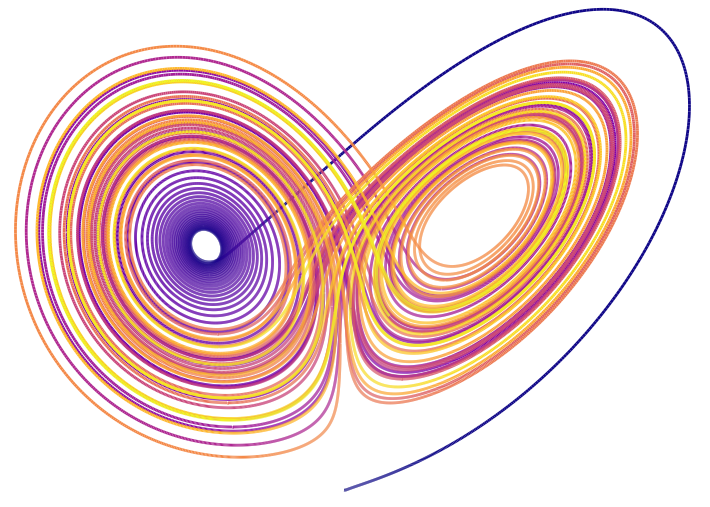
\includegraphics[scale=0.35]{graphics/attractor3.png}
				{\small \caption{Lorenz attraktori Runge-Kutta menetelmällä}}
			\end{figure}
		\end{column}
	\end{columns}
\end{frame}

\end{document}